\chapter{Konstrukcja}
	\section{Wybór mikrokontrolera}
	W przypadku robota autonomicznego istotną jego częścią jest jednostka logiczna, która nim steruje. Powinna być wystarczająco wydajna aby umożliwić szybkie podejmowanie decyzji na podstawie odczytów z czujników oraz stanu wewnętrznego robota. W przypadku braku zewnętrznego sterowania przez operatora, robot sam powinien unikać kolizji oraz decydować o kierunku poruszania się.
	
	Obecnie dostępnych jest wiele rodzajów mikrokontrolerów, a konkurencyjność zapewnia niskie ceny zakupu. To sprawia, że są one w zasięgu finansowym przeciętnego człowieka. Najbardziej rozpowszechnioną platformą jest seria Arduino \cite{arduinoFramework}. Posiada ona dużą ilość użytkowników i dzięki temu można łatwo uzyskać wsparcie w przypadku problemu z platformą. Przykładową gotową płytką z 8-bitowym procesorem ATmega2560 jest Arduino Mega \ref{fig:mikrokontrolery}. Posiada zegar o maksymalnej częstotliwości 16Mhz, 54 piny cyfrowe (w tym 15 PWM i 6 wspierających przerwania), 16 pinów analogowych i 6 timerów. Cena w przypadku nieoryginalnej wersji płytki wynosi około 7\$ (28zł)
	
	Kolejnym przykładem rodziny mikrokontrolerów z dużym wsparciem użytkowników jest Raspberry Pi. Przykładową płytką jest Raspberry Pi 4 model B \ref{fig:mikrokontrolery}. Posiada 4-rdzeniowy, 64-bitowy procesor o taktowaniu GHz, od 1 do 4GB pamięci RAM oraz 40 pinów cyfrowych. Zaletą tej płytki jest jej wysoka wydajność i możliwość wgrania pełnoprawnego systemu operacyjnego. Przykładem może być system operacyjny Rasbian \cite{raspbian}. Jest to wersja Linuxa podobna do systemu Debian. Minusem jest cena która dla najnowszego modelu wynosi około 50\$ (200zł) natomiast dla starszej wersji około 40\$ (160zł).

	\begin{figure}[h]
		\centering
		\begin{tabular}{@{}ll@{}}
			a) & b) \\
			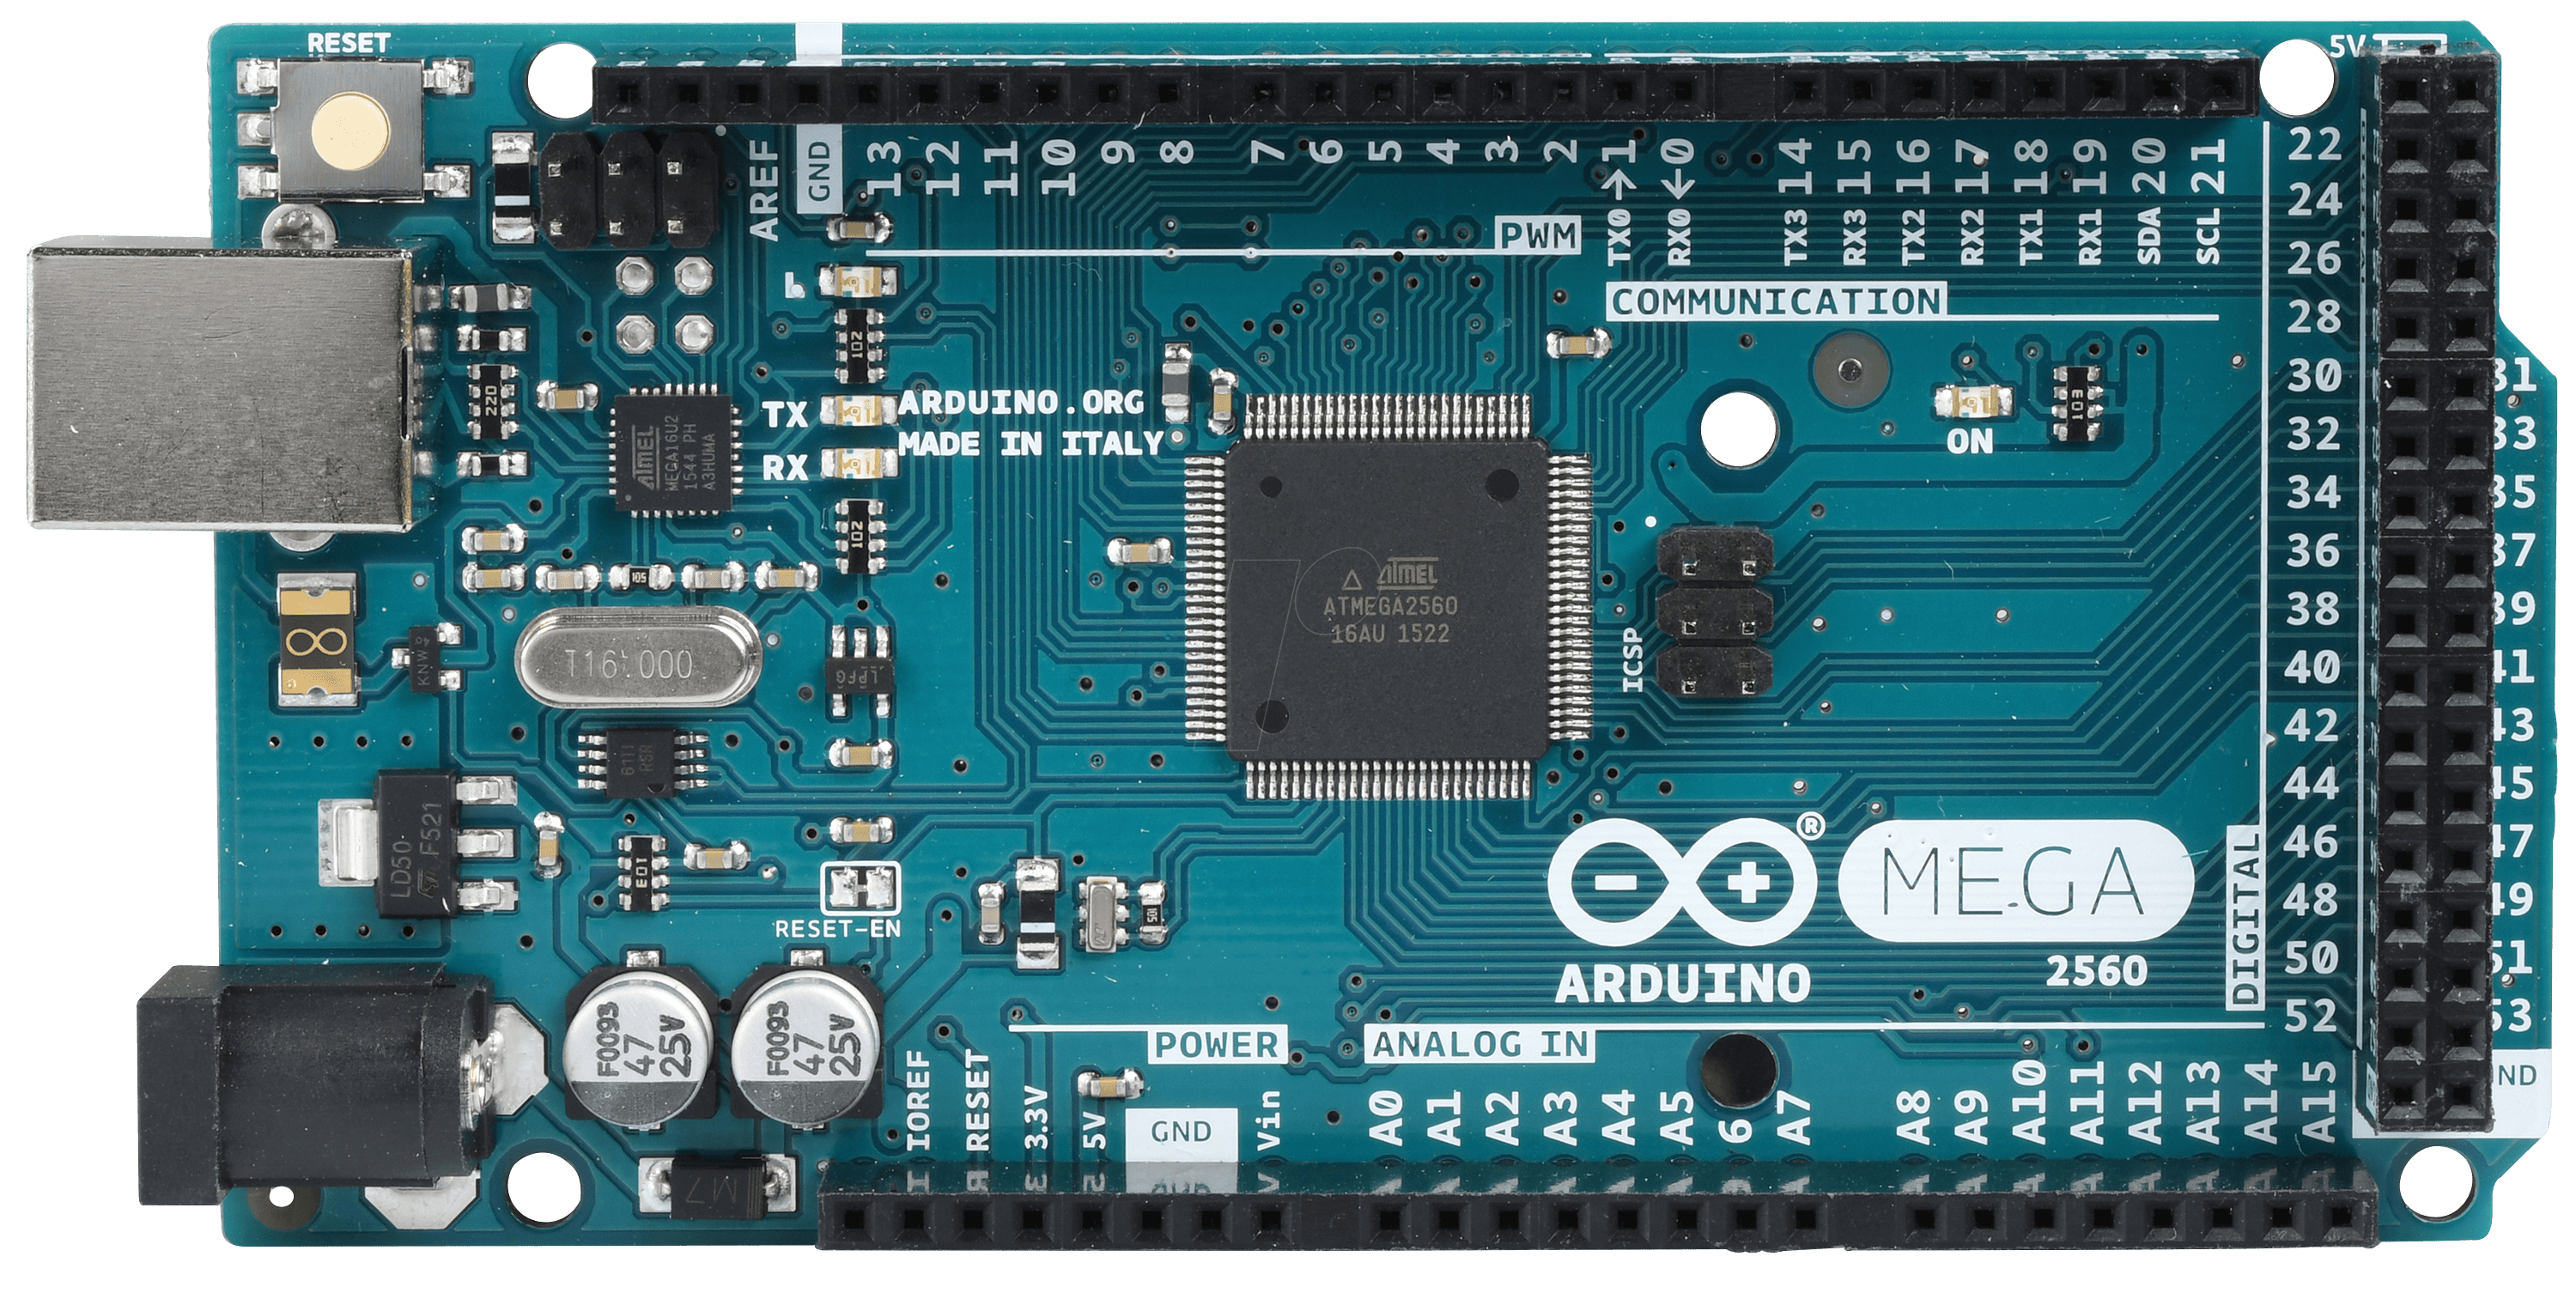
\includegraphics[width=0.5\textwidth]{rysKonstrukcja/Mega.png} & 
			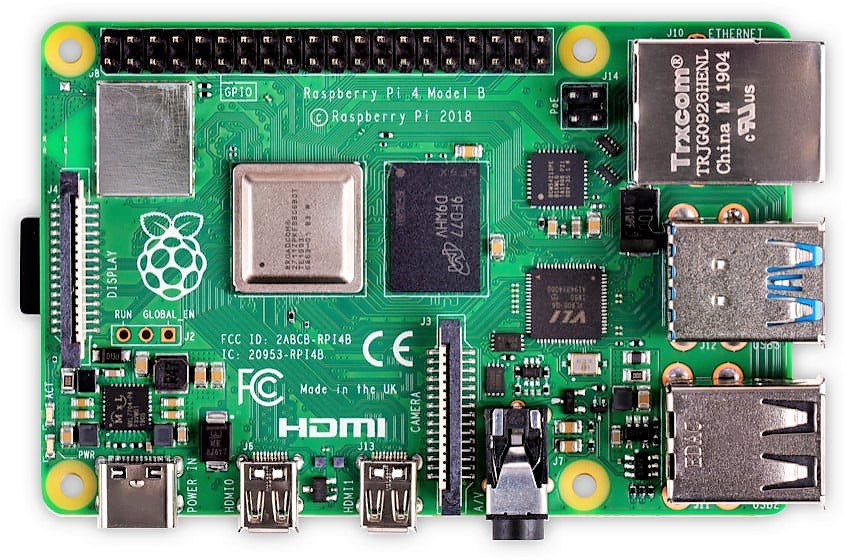
\includegraphics[width=0.5\textwidth]{rysKonstrukcja/raspberry.jpg} \\
		\end{tabular}
		\caption{Mikrokontrolery: a) Arduino Mega, b) Raspberry Pi}
		\label{fig:mikrokontrolery}
	\end{figure}

	Trzecią alternatywą łączącą pozytywy obu wymienionych wcześniej platform są mikrokontrolery STM32. Przykładową płytką jest STM32F103 Blue Pill \ref{fig:bluepillPlytka}. Posiada 32 konfigurowalne piny, 16 może obsługiwać zewnętrzne przerwania, 10 pinów połączonych z przetwornikiem ADC. Dodatkowo 18 może pracować z napięciem 5V (sam procesor pracuje na napięciu 3.3V) co może być przydatne zważywszy na fakt, że większa część gotowych modułów pracuje w logice 5V. Procesor wyposażony jest również w kontroler DMA, który pozwala na pomiary ADC oraz komunikację bez użycia procesora. Maksymalna nominalna częstotliwość taktowania wynosi 72MHz i dzięki pętli PLL może być łatwo konfigurowana. W przypadku niewielkiego braku mocy obliczeniowej istnieje możliwość łatwego overclockingu do 128MHz kosztem braku komunikacji przez USB. Procesor wyposażony jest także w 4 timery 16-bitowe, 4-kanałowe. Posiada także kilka możliwości wyboru API. Od wysokopoziomowego STM32duino, opartego na wspomnianym wcześniej Arduino, przez HAL oraz starsze SPL kończąc na systemie czasu rzeczywistego FreeRTOS \cite{FreeRTOS}. Ogromnym plusem jest niska cena. Płytka kosztuje około 1.5\$ (6zł).

	\begin{figure}[h]
		\centering
		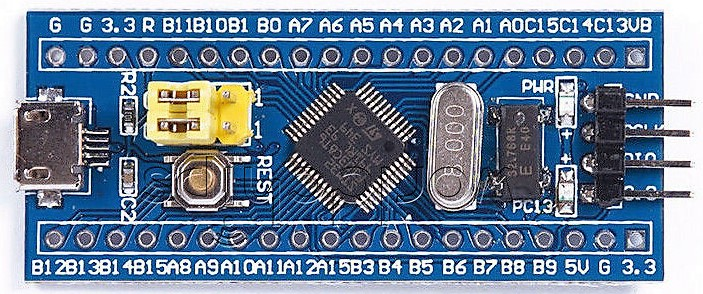
\includegraphics[width=0.8\textwidth]{rysKonstrukcja/bluepill.jpg} 
		\caption{Mikrokontroler STM32F103 Blue Pill}
		\label{fig:bluepillPlytka}
	\end{figure}
	
	Uwzględniając wskazane powyżej informacje wybrano płytkę STM32F103 Blue Pill. Zapewnia doby bilans między ilością peryferiów i wydajnością w porównaniu do pozostałych możliwości. Dodatkowo cechuje się najniższą ceną zakupu.
	
	\section{Pomiar odległości}
	
	Do orientacyjnego pomiaru odległości od przeszkód został wykorzystany moduł z czujnikiem ultradźwiękowym HC-SR04 \ref{fig:HCSR04}. Czujnik pozwala na pomiar odległości w zakresie \SI{2}{} --  \SI{400}{\centi\meter} z rozdzielczością \SI{0.3}{\centi\meter}. W trakcie projektowania brano pod uwagę, że na pomiar wpływa również propagacja fal dźwiękowych. Dlatego uwzględniono dodatkowe czujniki wykrywające przeszkody.
	
	\begin{figure}[H]
		\centering
		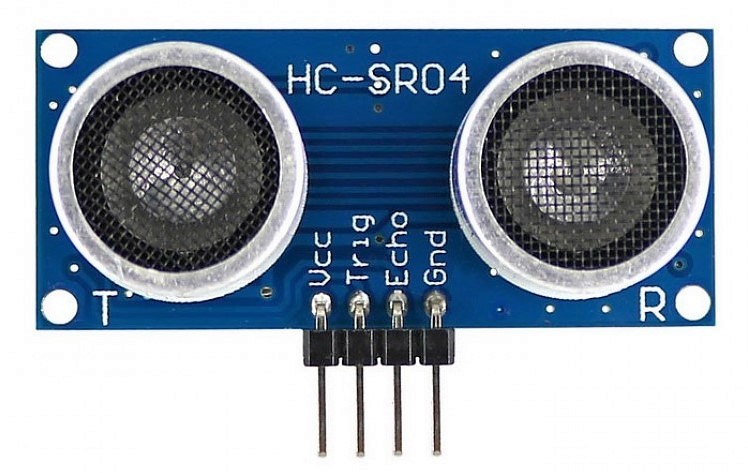
\includegraphics[width=0.4\textwidth]{rysKonstrukcja/HC-SR04.jpg} 
		\caption{Ultradźwiękowy moduł pomiaru odległości}
		\label{fig:HCSR04}
	\end{figure}

	Aby dokonać pomiaru czujnikiem należy na wejście Trig podać stan wysoki na co najmniej \SI{10}{\micro\second}. Moduł wysyła wtedy 8 ultradźwiękowych fal o częstotliwości \SI{40}{\kilo\hertz}. Po odebraniu pomiaru na pinie Echo pojawia się stan wysoki. W zależności od odległości od wykrytej przeszkody czas trwania wynosi od \SI{150}{\micro\second} do \SI{22}{\milli\second}. Jeśli nie wykryto przeszkody, czas stanu wysokiego wynosi \SI{38}{\milli\second}. Odległość w centymetrach można obliczyć korzystając z uproszczonej zależności \ref{eq:OdlegloscOdPrzeszkody}.
	
	\begin{equation}\label{eq:OdlegloscOdPrzeszkody}
		d = \unit[\frac{t}{58}]{cm}
	\end{equation}
	gdzie t - czas stanu wysokiego na pinie Echo w \SI{}{\micro\second}.
	
\chapter{Wstęp teoretyczny}
\texttt{Robot mobilny} - robot, który potrafi zmieniać swoje położenie w przestrzeni. Może być robotem autonomicznym, czyli takim który realizując swoje zadanie porusza się bezkolizyjnie w wyznaczonym środowisku oraz robi to bez ingerencji operatora.
Roboty mobilne można podzielić na kategorie przedstawione w tabeli~\ref{tab:kategorieRobotow}.
\begin{table}[htb] \small
	\centering
	\caption{Kategorie robotów mobilnych}
	\label{tab:kategorieRobotow}
	\begin{tabularx}{\linewidth}{|c|c|X|p{6cm}|} \hline\
		Narzędzie & Wersja & Opis & Adres \\ \hline\hline
		MiKTeX & 2.9 & Zalecana jest instalacja \texttt{Basic MiKTeX} z dystrubucji 32 lub 64 bitowej. Brakujące pakiety będą się doinstalowywać podczas kompilacji projektu. &
		\url{http://miktex.org/download} \\ \hline
		TexnicCenter & 2.02 &  Można pobrać 32 lub 64 bitową wersję & \url{http://www.texniccenter.org/download/} \\ \hline
		SumatraPDF & 3.1.1 & Można pobrać 32 lub 64 bitową wersję & \url{http://www.sumatrapdfreader.org/download-free-pdf-viewer.html} \\ \hline
		JabRef & 3.3 & Można pobrać 32 lub 64 bitową wersję & \url{http://www.fosshub.com/JabRef.html} \\ \hline
	\end{tabularx}
\end{table}
%%%
%%%Uwaga: tytuł powinien zmieścić się w okienku kolorowej okładki (którą
%%%powinna dostarczyć uczelniana administracja). Proszę posterować
%%%parametrami, aby "wpasować" w okienko własny tekst.
%%%
%%%Do ASAPa należy wprowadzić pracę dyplomową/projekt inżynierski w pliku o nazwie:
%%%
%%%W04_[nr albumu]_[rok kalendarzowy]_[rodzaj pracy] (szczegółowa instrukcja pod adresem asap.pwr.edu.pl)
%%%
           %%%Przykładowo:
        %%%­W04_123456_2015_praca inżynierska.pdf     - praca dyplomowa inżynierska
        %%%W04_123456_2015_projekt inżynierski.pdf   - projekt inżynierski
        %%%W04_123456_2015_praca magisterska.pdf  - praca dyplomowa magisterska
%%%
              %%%rok kalendarzowy ? rok realizacji kursu „Praca dyplomowa” (nie rok obrony) 